\chapter{Methods}
\label{ch:methods}


%% -----------------------------------------------------------------------------
%% -----------------------------------------------------------------------------
\section{Original Dataset} 

A database of WGS reaction data was assembled and provided as Supplementary Materials by Odabasi et al. \cite{Odabasi_2014}. This data set is composed of 4,360 data points from 97 publications between 2002 and 2012. The Odabasi et al. explored trends in this data using data mining techniques including decision trees, ANNs and support vector machines. The data was organized and described categorically by support, primary metal and promoter metal attributes. The optimized NN, trained with MATLAB's neural network toolbox, predicted CO conversion. They report a training performance of $R^2$=0.972, MSE = 5.42 and a testing performance of $R^2$=0.905, MSE = 10.05 \cite{Odabasi_2014}. 

%% -----------------------------------------------------------------------------
%% -----------------------------------------------------------------------------
\section{Data Disqualification}
This study expands on the results of Odabasi et al. by developing an ANN with new attributes and outputs. Prior to ANN development, the original data was `cleaned' to remove data that did not align with the objectives of this project or the constraints defined. This process reduced the training data set from 4,360 instances to 1,499 instances. The removal of data is summarized in Table \ref{table:data cleaning}. Note that some instances violated two or more of the constraints discussed. Therefore, Table \ref{table:data cleaning} reports both the total number of data points that violate each constraint as well as the number of data points removed after each sequential constraint is applied. 

Because the water-gas shift reaction is often studied in the context of steam-reforming of methane, 223 instances used co-feeding of methane. To eliminate conditions with competing reaction pathways, these data points were removed from the training data set. Similarly, the 98 instances with an \ce{O2} co-feed were removed. 

To enable modeling with continuous chemical property descriptors (i.e., electronegativity and ionization energies) rather than categorical descriptors (identity of each catalyst compound), guidelines for maintaining consistency amongst catalyst types were developed. First, only single metal-oxide supports were considered. Thus, any instances with zeolite (ZEO), hydroxyapatite (HAP) or activated carbon (ACC) based supports were removed (149 data points). Additionally, 953 instances with mixed metal-oxide supports were removed. To maintain promoter consistency, only pure metal promoters were considered. Due to this cutoff, 21 data points with yttrium-stabilized zirconia (YSZ) promotion were removed from the dataset. 

	\begin{table}[ht]
		\centering
		\caption{Number of data points lost by each cleaning criteria}
		\label{table:data cleaning}
		\begin{tabular}{lccc}
		\textbf{Removal Criteria} & \textbf{\begin{tabular}[c]{@{}c@{}}Order\\ Independent\end{tabular}} & \textbf{\begin{tabular}[c]{@{}c@{}}Sequential\\ Removal\end{tabular}} & \textbf{\begin{tabular}[c]{@{}c@{}}Remaining\\ Data Points\end{tabular}} \\ \hline
		Original Data                        & -            & -           & 4360        \\
		ZEO Support                          & 66           & 66          & 4292        \\
		HAP Support                          & 58           & 58          & 4236        \\
		ACC Support                          & 25           & 25          & 4211        \\
		YSZ Promoter                         & 21           & 21          & 4190        \\
		\ce{CH4} Co-Feed                     & 223          & 223         & 3967        \\
		\ce{O2} Co-Feed                      & 98           & 32          & 3935        \\
		$\beta > 0.8$                        & 355          & 265         & 3670        \\
		$\beta < 0$                          & 124          & 66          & 3604        \\
		$\beta$ Not Calculable               & 177          & 176         & 3428        \\
		T \textless 150\si{\celsius}         & 173          & 118         & 3310        \\
		T \textgreater 350\si{\celsius}      & 730          & 440         & 2870        \\
		Mixed Support                        & 953          & 642         & 2228       
		\end{tabular}
	\end{table}


	% ---------------------------------------------------
	\subsection{Removal of Kinetic Data Near Equilibrium}
	To compare and predict intrinsic catalyst activity, the data was cleaned to eliminate any instances which may have been affected by equilibrium or transport limitations. Furthermore, some instances in the dataset indicated thermodynamically impossible behavior (i.e., conversion that is impossible due to limiting reactants). The thermodynamic consistency of each data point was evaluated by determining the $\beta$ value, where $\beta$ is derived by Equations \ref{eq:B_start} to \ref{eq:B_end}. For each instance, $\beta$ was determined using the primary metal loading, reaction temperature, total flowrate, CO conversion and NIST thermodynamic parameters \cite{NIST}. 

	For an irreversible reaction the reverse rate constant, $k_{rev}$, must be zero and therefore, $\beta = 0$. When a reversible reaction is at thermodynamic equilibrium, $\beta = 1$. Because relevant kinetic data must be determined in a region without thermodynamic limitations, only instances with  $0 < \beta < 0.8$ were retained. The resulting data distribution is given in Figure \ref{fig:Beta_dist}. 
	\begin{equation}
		rate = rate_{for} - rate_{rev} \label{eq:B_start}\end{equation}
	\begin{equation}
		rate = k_{for}[CO][H_2O] - k_{rev}[CO_2][H_2] \end{equation}
	\begin{equation}
		rate = k_{for}[CO][H_2O] \left(1 - \frac{k_{rev}[CO_2][H_2]}{k_{for}[CO][H_2O]}\right) \end{equation}
	\begin{equation}
		\beta = \frac{k_{rev}[CO_2][H_2]}{k_{for}[CO][H_2O]} = \frac{[CO_2][H_2]}{K_{eq}[CO][H_2O]} \end{equation}
	\begin{equation}
		rate = rate_{for}(1-\beta) \end{equation}
	\begin{equation}
		rate_{for} = \frac{rate}{1-\beta} \label{eq:B_end} \end{equation}

	\begin{figure}[ht]
	    \centering
	    \begin{subfigure}[b]{0.49\textwidth}
	        \centering
	        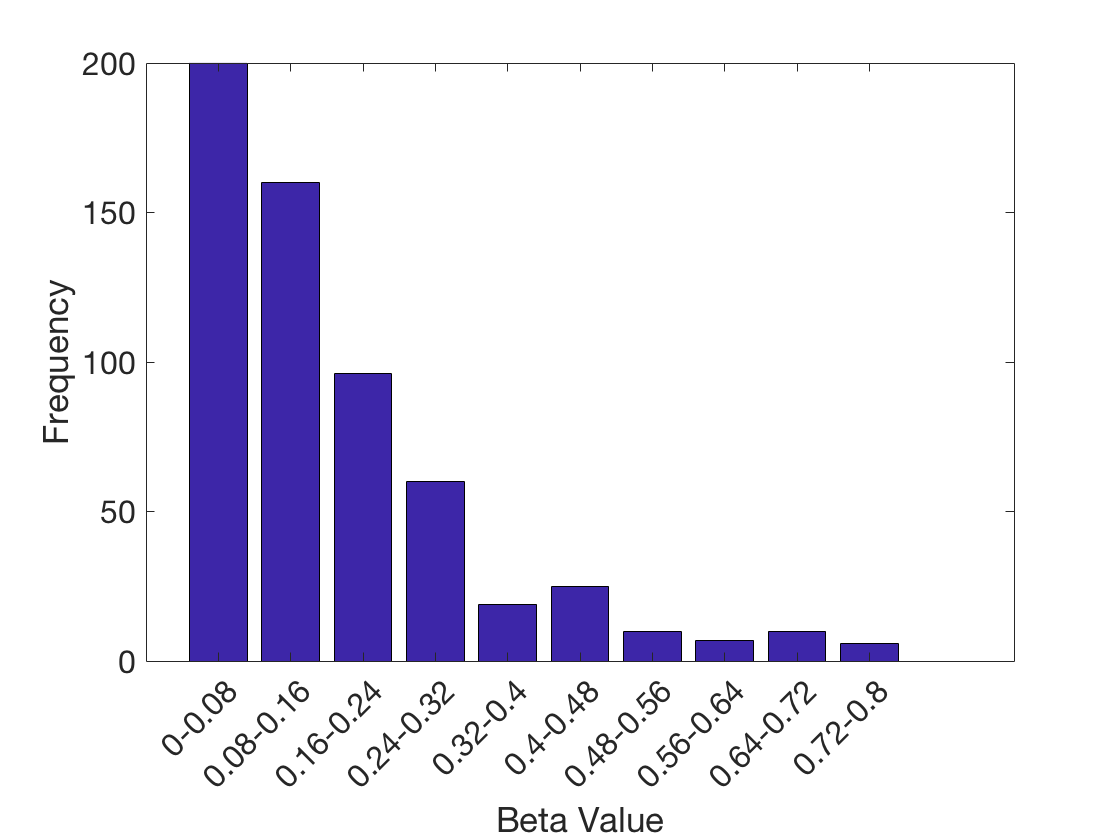
\includegraphics[width=\textwidth]{Methods/B_distribution.png}
	        \caption{$\beta$-value distribution histogram}
	        \label{fig:B dist histogram}
	    \end{subfigure}
	    \begin{subfigure}[b]{0.49\textwidth}
	        \centering
	        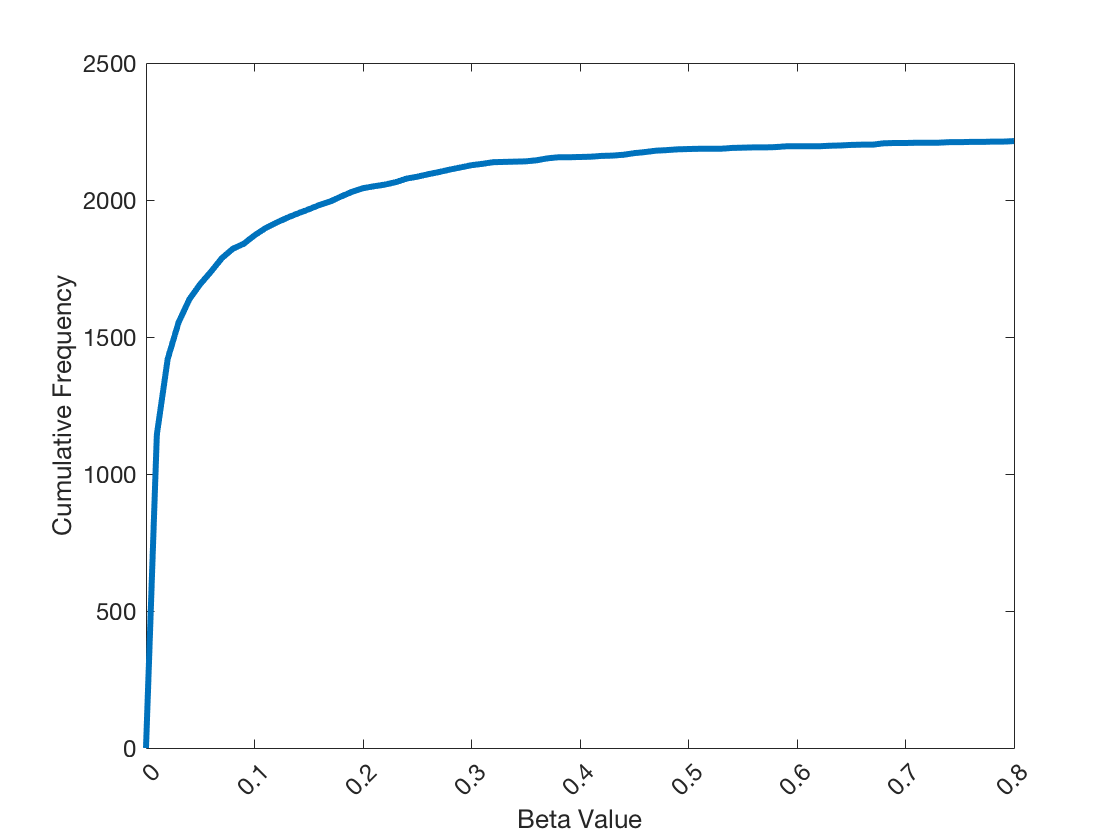
\includegraphics[width=\textwidth]{Methods/B_distribution_cum.png}
	        \caption{Cumulative $\beta$-value distribution}
	        \label{fig:B dist cum}
	    \end{subfigure}
	    \caption{Distribution of the $\beta$ values after removal of instances which did not have thermodynamic consistency or were near equilibrium}
	    \label{fig:Beta_dist}
	\end{figure}

	% ---------------------------------------------------
	\subsection{Limiting to LT-WGS}
	WGS reaction research has been reported over a large range of temperatures, but can be segregated into low-temperature (LT) WGS for 150\si{\celsius} to 350\si{\celsius} and high temperature (HT) WGS for reactions above 350\si{\celsius}. These two categories have distinctly different catalysts and proposed mechanisms. This work constrained the data set to instances within the low-temperature (LT) WGS reaction region, defined by reaction temperatures between 150\si{\celsius} and 350\si{\celsius}. 
	% Temperature Distribution Figures
	\begin{figure}[ht]
	    \centering
	    \begin{subfigure}[b]{0.49\textwidth}
	        \centering
	        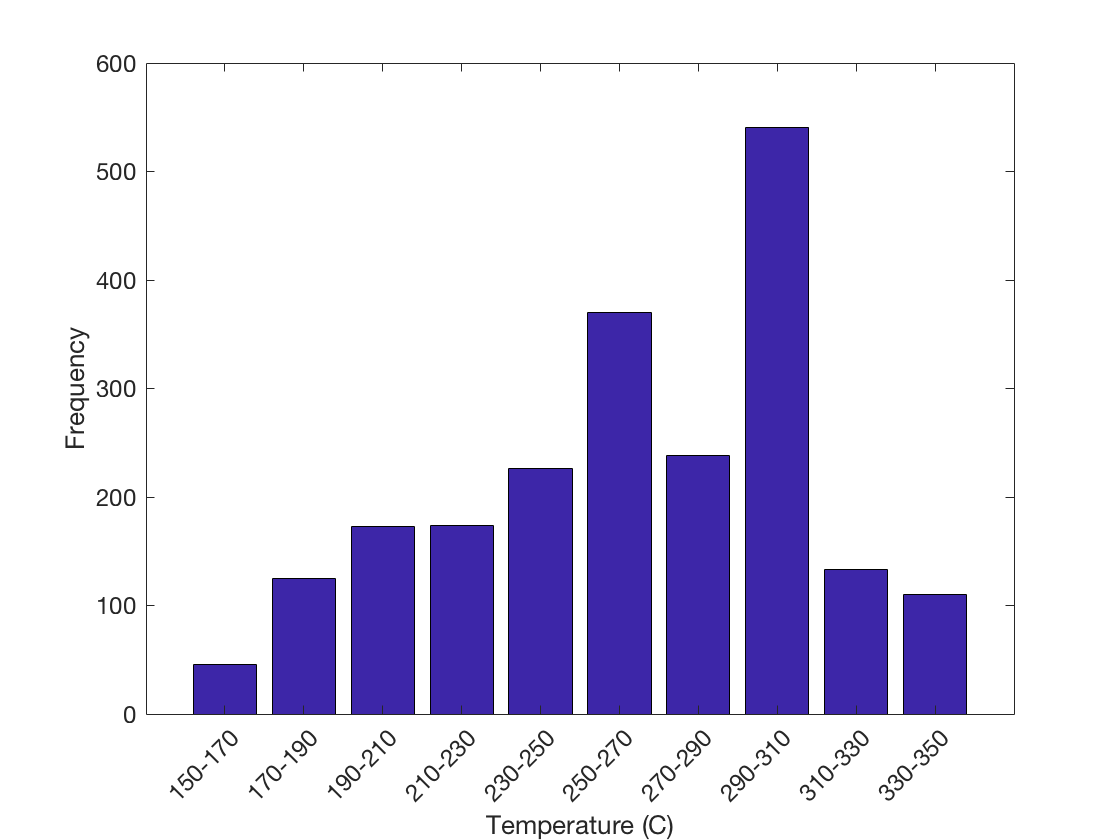
\includegraphics[width=\textwidth]{Methods/T_distribution.png}
	        \caption{Temperature distribution histogram}
	        \label{fig:T dis histogram}
	    \end{subfigure}
	    \begin{subfigure}[b]{0.49\textwidth}
	        \centering
	        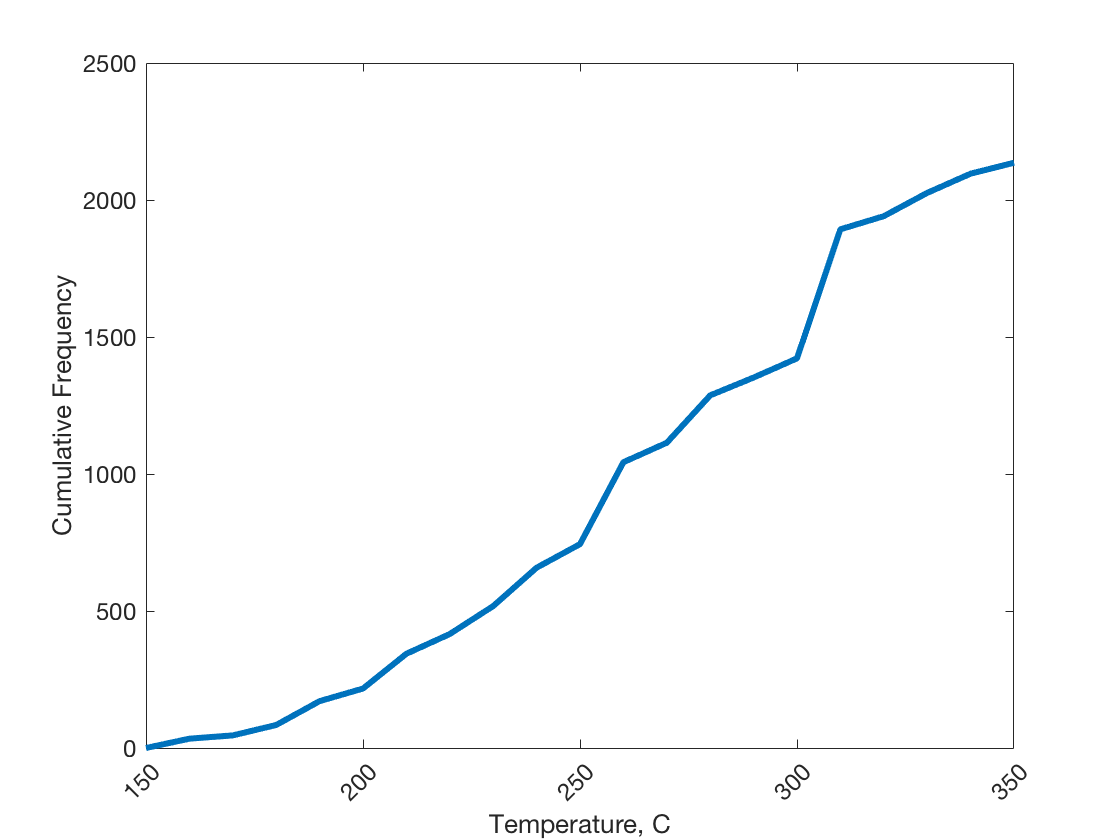
\includegraphics[width=\textwidth]{Methods/T_distribution_cum.png}
	        \caption{Cumulative temperature distribution}
	        \label{fig:T dist cum}
	    \end{subfigure}
	    \caption{Distribution of temperatures after data removal by  $\beta$ values and limiting to LT-WGS}
	    \label{fig:T_dist}
	\end{figure}


	% ---------------------------------------------------
	\subsection{Removing \ce{Au/CeO2} and \ce{Pt/CeO2} Instances}
	Early in the model development process, it was identified that outlying instances were consistently associated with \ce{Au/CeO2} and \ce{Pt/CeO2} catalysts. This finding had an important implication on the training performance, demonstrated in Table \ref{table: compare with AuPtCeO2}. As a results, 749 instances with \ce{Au/CeO2} or \ce{Pt/CeO2} catalysts were removed from the training data set, reducing the final size from 2,228 data points to 1,499 data points. This removal is further analyzed in the results section.
	\begin{table}[ht]
			\centering
			\caption{ANN Performance when trained with and without \ce{Au/CeO2} and \ce{Pt/CeO2}}
			\label{table: compare with AuPtCeO2}
			\begin{tabular}{l|cc}
				\textbf{Data Set}          & \textbf{$R^2$} & \textbf{MSE} \\ \hline
				With Au/CeO2 \& Pt/CeO2    & 0.91                  & 0.32         \\
				Without Au/CeO2 \& Pt/CeO2 & 0.95                  & 0.24         \\
				Difference                 & 0.03                  & 0.08        
				\end{tabular}
				\end{table}
% ---------------------------------------------------
\section{Data Normalization}
Training ANNs with vastly different attribute distributions delays the learning process and complicates initialization of the network \cite{Ioffe_2015}. Therefore, data normalization, or `feature scaling', is frequently used to achieve similar performance with a reduced number of iterations. All non-categorical features were scaled using the standardization equation, \ref{eq:standardization}, which is frequently used in machine learning \cite{Grus_2015}.
		\begin{equation}
			x' = \frac{x - \bar{x}}{\sigma}\label{eq:standardization}\end{equation}

The ANN output is the forward rate, given by equation \ref{eq:B_end}. Rate is defined as moles of \ce{CO} consumed per minute per mole of primary metal. The forward rate originally demonstrated a log-normal distribution, shown in figure \ref{fig:non-norm_dist}. This data distribution significantly impeded training and testing performance. To correct for this distribution, the natural logarithm of the forward rates was taken, normalizing the probability distribution to a zero mean, demonstrated in Figure \ref{fig:norm_dist}.
\begin{figure}[ht]
    \centering{}
    \begin{subfigure}[b]{0.48\textwidth}
        \centering
        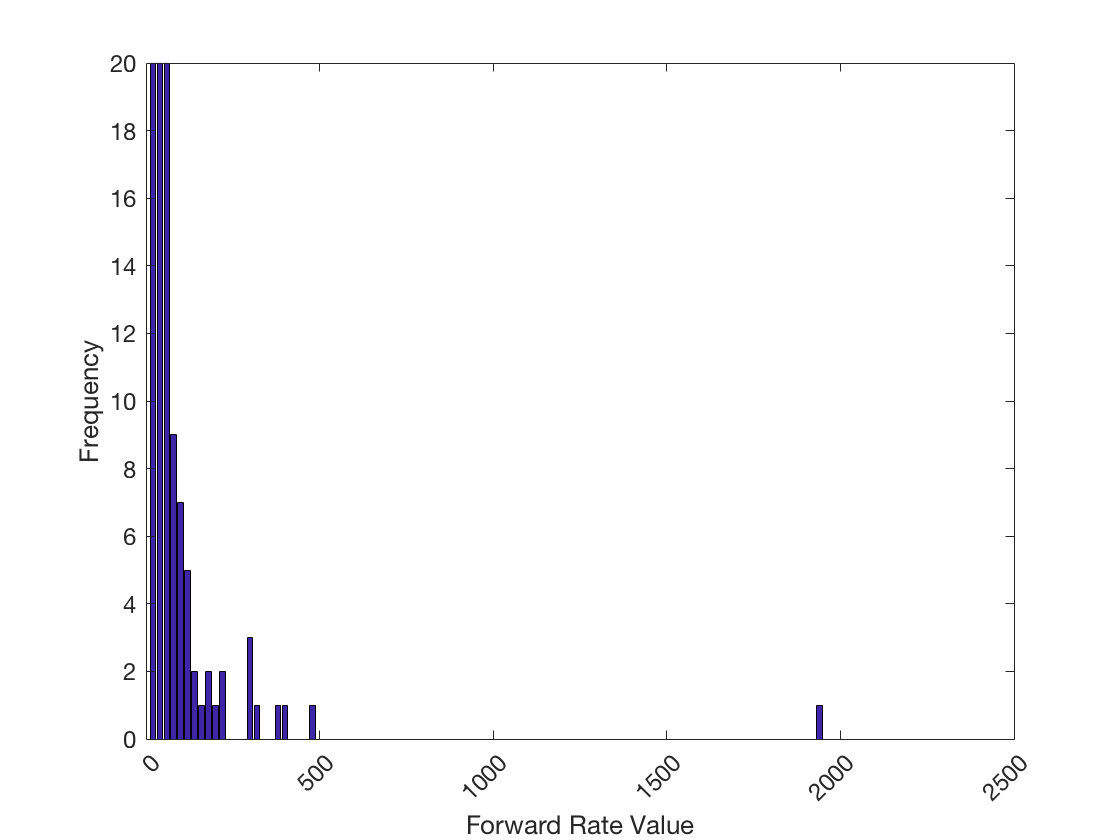
\includegraphics[width=\textwidth]{Methods/DataDistribution_nonNormalized_histogram.png}
    	\end{subfigure}
    \begin{subfigure}[b]{0.48\textwidth}
        \centering
        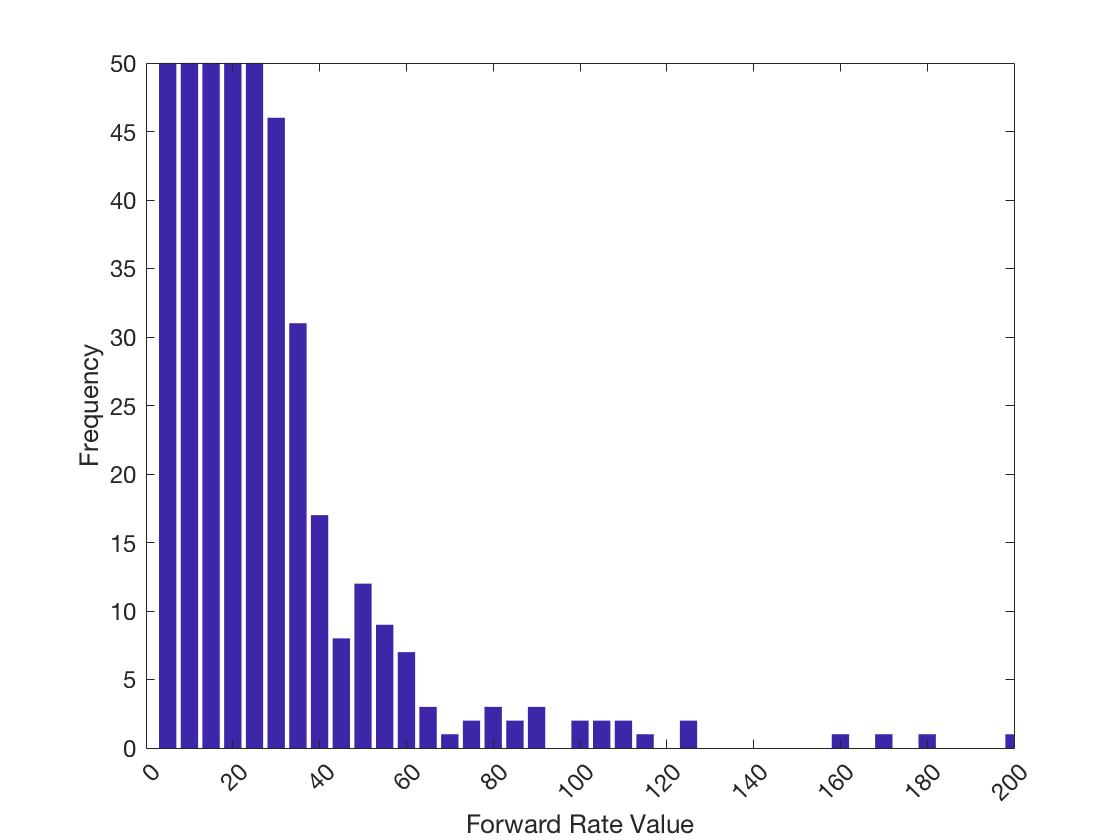
\includegraphics[width=\textwidth]{Methods/DataDistribution_nonNormalized_zoomed.png}
    	\end{subfigure}
    \caption{Histograms of forward rate distribution prior to normalizing}
    \label{fig:non-norm_dist}
	\end{figure}

\begin{figure}[ht]
	    \centering
        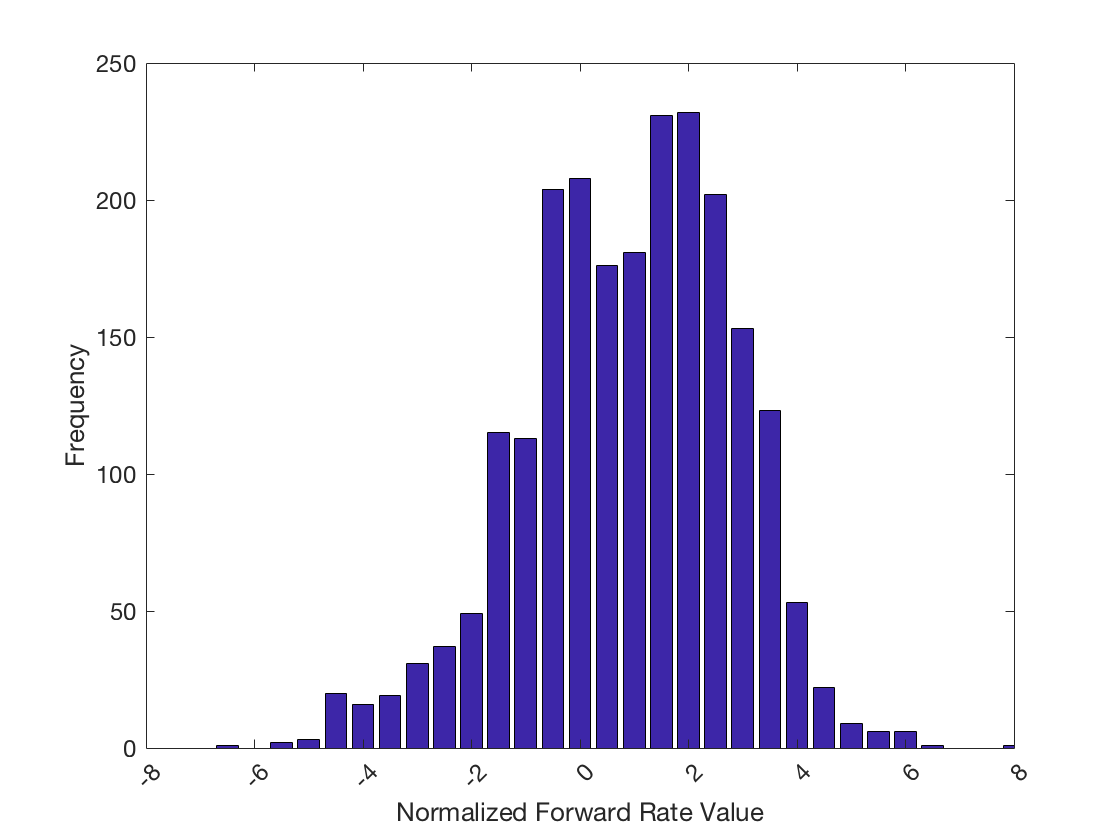
\includegraphics[width=0.48\textwidth]{Methods/DataDistribution_Normalized_histogram.png}
        \caption{Normalized forward rate histogram}
        \label{fig:norm_dist}
		\end{figure}

%% -----------------------------------------------------------------------------
%% -----------------------------------------------------------------------------
\section{Model Development}
The MATLAB Neural Network Toolbox was used to create and train ANNs. Specifically, the fitnet() function was used to define network architecture, backpropagation method and training performance parameters.

Overfitting is a significant consideration for ANN development. Overfitting occurs when a neural network receives too much training with the training data and thus, loses its ability to generalize for new instances or inputs. As a result, the error with respect to the training data is small but the error with respect to non-training data is much larger. Overfitting can be avoided by monitoring and controlling the training procedure through a process called `cross-validation' \cite{Kohavi_1995}. With cross-validation, the entire training set is iteratively, randomly divided into a training set and a validating set. The training set is used to train the ANN while the validation set is used to evaluate the network performance on a `blind' set of data. While the network is training, the error on both the training and the validation sets decreases. When overfitting begins, the error on the training set continues to decrease while the error on the validation set begins in increase. The MATLAB fitnet() tool uses k-fold cross validation to reduce overfitting of the ANN. k-fold cross validation is used to reduce variability, which averages the results over many rounds of dividing the data into different training and validating sets. 

For each ANN presented here, the original data set was first divided into model training data (80\%) and independent testing data (20\%). The model training data was then further divided by MATLAB's fitnet() function into a training data set (70\%), a validation data set (30\%) and used to develop an ANN. Therefore, the data divisions compound to 56\% for training, 24\% for validation and 20\% for testing. 

The fitnet() function was modified by increasing the maximum number of iterations to 2,500 and adjusting the backpropagation algorithm from the default Levenberg-Marquardt regularization to Bayesian regularization. Both of these adjustments improved model performance, as evaluated by the mean-squared error and the coefficient of determination. These training adjustments did not result in overfitting. Adjusting other parameters (maximum number of epochs, performance goal, learning rate and performance gradient) was explored and did not significantly improve model performance. The summary of model training parameters is provided in Table \ref{table:training params}. 
		\begin{table}[ht]
			\centering
			\caption{ANN Model Training Parameters}
			\label{table:training params}
			\begin{tabular}{l|l}
			\textbf{Parameter}    & \textbf{Specification}  \\ \hline
			Error Function        & Mean-squared error      \\
			Backpropagation       & Bayesian Regularization \\
			Maximum Iterations    & 2,500                   \\
			Training Data         & 56\% of total data      \\
			Cross Validation Data & 24\% of total data      \\
			Testing Data          & 20\% of total data     
			\end{tabular}
			\end{table}

The performance of the ANN was then evaluated with the independent testing data using both \(R^2\) and the MSE. Note that due to the k-means cross validation procedure used by MATLAB's fitnet() function, the testing performance provided by the fitnet() function is consistently larger than the independently determined error. All results presented henceforth are determined with the independent testing data unless otherwise noted. 

%% -----------------------------------------------------------------------------
%% -----------------------------------------------------------------------------
\section{Attribute Determination}
Predictions made by ANNs are limited to interpolation within the domain space. Therefore, representing the data to maximize the domain space also maximizes the types of catalysts that can be evaluated using the ANN. A critical modification was migrating the data from the originally categorical representation to a continuous representation that accurately captured complex relationships between attributes. This adjustment allows predictions to be made for catalysts that were not explicitly included in the training data set, but whose descriptors lie within the defined domain. 

To determine the most relevant features in describing the training data, many descriptors were compared for each component of the catalyst (support, primary metal, promoter). An ANN was trained according to the algorithm below using each attribute individually. After multiple training cycles, the average mean squared error (MSE) and $R^2$ error was reported, as shown in Table \ref{table: BE_comparison}. The `best' attribute was determined to be that which resulted in the least error (smallest MSE and largest $R^2$). Thus, the final ANN incorporated the attributes which independently improved ANN testing performance. The following algorithm was used to determine the average MSE and $R^2$: 

		\begin{quote}
		Randomize the data $m$ times\\
		For each randomization, train $n$ ANNs\\
		For each ANN evaluate performance (testing $R^2$ and MSE)\\
		Record the best performance from the $n$ trained ANNs\\
		Report the average error of the best performance over $m$ randomizations 
		\end{quote}

	\subsection{Primary Metal Descriptors}
	To build the most complete domain, a descriptor is needed to relate the separate active noble metals to one another. A well-understood descriptor is the energy of a reactive species binding to the surface of the metal. It has been demonstrated that activity is highly correlated to optimizing the binding energy of a surface \cite{Greeley_2016}. For this case study, the binding energies of C, O, H, CO and OH were considered, as each is expected to be present on the catalyst surface and play a prevalent role in the WGS mechanism \cite{Gokhale_2008}.

	For this project, the adsorption energy of carbon on the specified surface of each noble metal was used as the active metal descriptor, given in Table \ref{table:BEs}. Relating the surfaces with a descriptor that lies on a continuous scale allows predictions to be made for materials that were not included in the training dataset. All adsorption energies were taken from a single publication by Herron et al. to ensure consistency \cite{Herron_2014}. 
			\begin{table}[ht]
				\centering
				\caption{Binding energy (eV) of relevant species on noble metal surfaces \cite{Herron_2014}}
				\label{table:BEs}
				\begin{tabular}{l|ccccc}
				\textbf{Surface} & \textbf{CO} & \textbf{O} & \textbf{C} & \textbf{H} & \textbf{OH} \\ \hline
				Au(111)          & 0.3         & -1.94      & -3.06      & -1.84      & -1.06       \\
				Cu(111)          & -0.33       & -3.58      & -3.75      & -2.2       & -2.13       \\
				Pt(111)          & -1.34       & -3.18      & -5.81      & -2.57      & -1.65       \\
				Pd(111)          & -1.49       & -3.14      & -5.62      & -2.62      & -1.65       \\
				Ir(111)          & -1.52       & -4.14      & -6.46      & -2.61      & -2.12       \\
				Rh(111)          & -1.51       & -4.13      & -5.67      & -2.64      & -2.14       \\
				Ru(0001)         & -3.47       & -4.73      & -6.16      & -2.75      & -2.64      
				\end{tabular}
				\end{table}

	Binding energies are typically highly correlated, and therefore, the primary metal should be sufficiently described with a single binding  energy \cite{Greeley_2016}. To determine the adsorbate that best describes the primary metal, ANNs were trained using one of the five possible attributes listed in Table \ref{table:BEs} and the algorithm presented with $m = 5$ and $n = 25$. Both the MSE and the $R^2$ error, reported in Table \ref{table: BE_comparison} were determined with independent testing data and used to identify to optimum adsorbate for use as a primary metal descriptor. Based on the results given in Table \ref{table:BEs}, using carbon as the adsorbate produced the least error in the model. 
			\begin{table}[ht]
				\centering
				\caption{Comparison of binding species for primary metal attribute}
				\label{table: BE_comparison}
				\begin{tabular}{ccc}
				\textbf{\begin{tabular}[c]{@{}l@{}}Binding\\ Species\end{tabular}} & \textbf{MSE} & \textbf{$R^2$} \\ \hline
				C          & 0.49         & 0.87                         \\
				CO         & 0.55         & 0.86                         \\
				H          & 0.56         & 0.85                         \\
				O          & 0.58         & 0.85                         \\
				OH         & 0.59         & 0.85                        
				\end{tabular}
				\end{table}

	\subsection{Support Attributes}
	A similar procedure was used to determine the best support attributes. Only single metal oxide supports were considered. Each support was described by the chemical properties of the metal or metalloid. Non-metal oxide supports, such as zeolite, hydroxyapatite and activated carbon were removed from the data set as described. For all remaining supports, the following chemical descriptors were explored: ionization energy, reduction potential, electronegativity, most reduced state and most oxidized state. The value of each attribute for each support is given in appendix \ref{table: Supp Properties}. The analysis results are listed in Table \ref{table: supports}. The first ionization energy and electronegativity were chosen as the most meaningful support attributes. 
			\begin{table}[ht]
				\centering
				\caption{Comparison of chemical properties for support attributes}
				\label{table: supports}
				\begin{tabular}{lll}
				\textbf{Support Descriptor} & \textbf{MSE} & \textbf{$R^2$} \\ \hline
				First Ionization Energy     & 0.26         & 0.93                         \\
				Electronegativity           & 0.29         & 0.93                         \\
				MW of Metal Oxide           & 0.32         & 0.92                         \\
				MW of Metal                 & 0.33         & 0.91                         \\
				Highest Oxidation State     & 0.36         & 0.91                         \\
				Reduction Potential         & 0.38         & 0.90                         \\
				Lowest Reduction State      & 0.39         & 0.90                        
				\end{tabular}
				\end{table}
	\subsection{Promoter Attributes}
	Chemical properties were also chosen for promoter attributes. Ionization energies, electronegativity, atomic radius, covalent radius, most oxidized state, most reduced state, ionic radius, reduction potential and charge/ionic radius were explored as descriptors. The value of each attribute for each promoter is given in appendix \ref{table:promoter props}. Using the algorithm described with $m = 5$ and $n = 25$, the best promoter attributes were determined. For these trials, the primary metal descriptor was $BE_C$ and the support descriptors were first ionization energy and electronegativity. From the results in Table \ref{table: promoter Att}, electronegativity and charge/ionic radius were chosen as promoter attributes. 

	\begin{table}[ht]
		\centering
		\caption{Comparison of chemical properties for promoter attributes}
		\label{table: promoter Att}
		\begin{tabular}{lll}
		\textbf{Promoters}      & \textbf{$R^2$} & \textbf{MSE} \\ \hline
		Charge/Ionic Radius     & 0.93                         & 0.275        \\
		Electronegativity       & 0.92                         & 0.296        \\
		First Ionization Energy & 0.92                         & 0.300        \\
		Redox                   & 0.92                         & 0.302        \\
		Molecular Weight        & 0.92                         & 0.306        \\
		Most Reduced State      & 0.92                         & 0.312        \\
		Most Oxidized State     & 0.92                         & 0.315        \\
		Covalent Radius         & 0.88                         & 0.438       
		\end{tabular}
		\end{table}

	\subsection{Resulting Domain Space}
	The domain space after cleaning the data set and determining the optimum attributes is given in \ref{table: domain}. This corresponds to instances with the supports, primary metals and promoters listed in Table \ref{table: domain elements}. The remaining categorical synthesis methods are incipient wetness impregnation (IWI), wet impregnation (WI), co- impregnation (CI), sequential impregnation (SI), homogenous deposition precipitation (HDP), flame spray pyrolysis (FSP), deposition precipitation (DP). 

			\begin{table}[ht]
					\centering
					\caption{Domain of the ANN after cleaning and attribute selection}
					\label{table: domain}
					\begin{tabular}{llcc}
					\textbf{Attribute}                     &                 & \textbf{\begin{tabular}[c]{@{}c@{}}Minimum\\ Value\end{tabular}} & \textbf{\begin{tabular}[c]{@{}c@{}}Maximum\\ Value\end{tabular}} \\ \hline
					Binding Energy Carbon                  & (eV)            & -6.46             & -3.06           \\
					Primary Metal Loading                  & (wt\%)          & 0.1               & 39.8            \\
					Promoter, Charge/Ionic Radius          & (charge/pm)     & 0.06 (0)          & 1.52            \\
					Promoter, Electronegativity            & (Pauling Scale) & 0.79 (0)          & 1.91            \\
					Promoter Loading                       & (wt\%)          & 0                 & 20              \\
					Support Metal, First Ionization Energy & (kJ/mol)        & 534.4              & 786.5            \\
					Support Metal, Electronegativity       & (Pauling Scale) & 1.1               & 1.9             \\
					Synthesis Method                       &                 & \multicolumn{2}{c}{IWI, WI, CI, SI, HDP, FSP, DP}                                                                                   \\
					Calcination Temperature                & (Celsius)       & 25                & 650             \\
					Calcination Time                       & (hours)         & 0                 & 10              \\ \hline
					Reaction Temperature                   & (Kelvin)        & 423               & 623             \\
					Reactant Feed, \ce{H2} vol\%                &                 & 0                 & 60              \\
					Reactant Feed, \ce{CO} vol\%                &                 & 0.2               & 12              \\
					Reactant Feed, \ce{H2O} vol\%               &                 & 2                 & 60              \\
					Reactant Feed, \ce{CO2} vol\%                &                 & 0                 & 15              \\
					Time on Stream                         & (min)           & 0.8               & 4314            \\
					Total Inlet Flowrate/Catalyst Mass     & (mL/min/g)      & 0.028             & 17.6           
					\end{tabular}
					\end{table}

				\begin{table}[ht]
					\centering
					\caption{Catalyst components in the domain}
					\label{table: domain elements}
					\begin{tabular}{ccc}
					\textbf{Supports} & \textbf{Primary Metals} & \textbf{Promoters} \\ \hline
					\ce{CaO}               & Cu                      & Li                 \\
					\ce{Y2O3}              & Ru                      & Na                 \\
					\ce{TiO2}              & Rh                      & K                  \\
					\ce{ZrO2}              & Pd                      & Rb                 \\
					\ce{HfO2}              & Ir                      & Cs                 \\
					\ce{MnO}               & Pt                      & Ca                 \\
					\ce{Fe2O3}             & Au                      & Sr                 \\
					\ce{Co3O4}             &                         & Y                  \\
					\ce{La2O3}             &                         & Ti                 \\
					\ce{CeO2}              &                         & Zr                 \\
					\ce{ThO2}              &                         & Cr                 \\
					\ce{Al2O3}             &                         & Mn                 \\
					\ce{SiO2}              &                         & Fe                 \\
					                       &                         & Co                 \\
					                       &                         & Ni                 \\
					                       &                         & Re                 \\
					                       &                         & Zn                 \\
					                       &                         & La                 \\
					                       &                         & Ce                 \\
					                       &                         & Nd                 \\
					                       &                         & Ho                 \\
					                       &                         & Er                 \\
					                       &                         & Tm                
					\end{tabular}
					\end{table}

%% -----------------------------------------------------------------------------
%% -----------------------------------------------------------------------------
\section{Determining Architecture}
A critical step in ANN development is determining the `optimum' architecture for the ANN. While no `rules' or heuristics exist for specifying how to determine this, it does depend on the amount of training data, the number of inputs and the complexity of the problem. For this project, all architectures explored had either one or two hidden layers with the second hidden layer being equal to or smaller than the first hidden layer. Furthermore, a given network should have twice as many training data points as it does network weights, to decrease the risk of overfitting. Due to the large size of the training data set, this was not a concern for the architectures explored. For each ANN, the optimum architecture was determined with a `brute force' search approach. In other words, a large number of ANNs were trained and evaluated, using the algorithm described with $m = 5$ and $n = 5$ for a total of 25 trained ANNs per architecture. For each architecture, the overall `best' and the average MSE was reported. After completing the broad architecture search given in Table \ref{table: archs 1}, a more rigorous comparison was performed with $m = 5$ and $n = 20$ for the top three architectures identified with the broad search. These results are presented in \ref{table: archs 2}. The results in both searches agree that the optimum ANN architecture has six neurons in the first hidden layer and two neurons in the second hidden layer. Thus, the final ANN has 23 inputs, one for each attribute and synthesis method in \ref{table: domain}, six hidden neurons in the first layer, two neurons in the second hidden layer and a single output for the $ln(rate_{forward})$. 
		
		\begin{table}[ht]
			\centering
			\caption{Optimization of ANN Architecture}
			\label{table: archs 1}
			\begin{tabular}{ccccc}
			\textbf{\begin{tabular}[c]{@{}c@{}}1st Hidden\\ Layer\end{tabular}} & \textbf{\begin{tabular}[c]{@{}c@{}}2nd Hidden\\ Layer\end{tabular}} & \textbf{\begin{tabular}[c]{@{}c@{}}Weights in\\ Network\end{tabular}} & \textbf{\begin{tabular}[c]{@{}c@{}}Average\\ MSE\end{tabular}} & \textbf{\begin{tabular}[c]{@{}c@{}}Best\\ MSE\end{tabular}} \\ \hline
			5      & 0        & 120          & 0.47      & 0.35     \\
			5      & 1        & 121          & 0.39      & 0.27     \\
			5      & 2        & 127          & 0.52      & 0.36     \\
			5      & 3        & 133          & 0.44      & 0.25     \\
			5      & 4        & 139          & 0.49      & 0.27     \\ \hline
			6      & 0        & 144          & 0.43      & 0.33     \\
			6      & 1        & 145          & 0.47      & 0.38     \\
			6      & 2        & 152          & 0.35      & 0.23     \\
			6      & 3        & 159          & 0.43      & 0.25     \\
			6      & 4        & 166          & 0.39      & 0.28     \\ \hline
			7      & 0        & 168          & 0.43      & 0.25     \\
			7      & 1        & 169          & 0.60      & 0.34     \\
			7      & 2        & 177          & 0.41      & 0.26     \\
			7      & 3        & 185          & 0.58      & 0.34     \\
			7      & 4        & 193          & 0.37      & 0.30     \\ \hline
			8      & 0        & 192          & 0.36      & 0.23     \\
			8      & 1        & 193          & 0.43      & 0.27     \\
			8      & 2        & 202          & 0.47      & 0.37     \\
			8      & 3        & 211          & 0.53      & 0.28     \\
			8      & 4        & 220          & 0.56      & 0.37     
			\end{tabular}
			\end{table}
		
		\begin{table}[ht]
			\centering
			\caption{Rigorous optimization of ANN architectures}
			\label{table: archs 2}
			\begin{tabular}{ccccc}
			\textbf{\begin{tabular}[c]{@{}c@{}}1st Hidden\\ Layer\end{tabular}} & \textbf{\begin{tabular}[c]{@{}c@{}}2nd Hidden\\ Layer\end{tabular}} & \textbf{\begin{tabular}[c]{@{}c@{}}Weights in\\ Network\end{tabular}} & \textbf{\begin{tabular}[c]{@{}c@{}}Average\\ MSE\end{tabular}} & \textbf{\begin{tabular}[c]{@{}c@{}}Best\\ MSE\end{tabular}} \\ \hline
			5         & 1          & 121         & 0.41         & 0.31               \\
			6         & 2          & 152         & 0.40         & 0.19               \\
			8         & 0          & 192         & 0.38         & 0.29              
			\end{tabular}
			\end{table}

